\documentclass[11pt, a4paper]{article}
\usepackage[margin=2cm]{geometry}
\usepackage{svg}
\usepackage{setspace}
\usepackage[hidelinks]{hyperref}
\usepackage[toc,title]{appendix}
\usepackage{graphicx}
\usepackage{rotating}
\usepackage{afterpage}
\usepackage{adjustbox}


\usepackage[
backend=biber,
style=apa,
url=false,
doi=true,
isbn=false
]{biblatex}
%\usepackage{textcomp}
\usepackage{phonetic}
\usepackage{fontawesome5}
\usepackage{textcomp, xspace}
\newcommand\la{\textlangle\xspace}  % set up short-form macros
\newcommand\ra{\textrangle\xspace}

\newenvironment{itquote}
  {\begin{quote}\itshape}
  {\end{quote}\ignorespacesafterend}

\addbibresource{literature.bib}
%%%%%%%%%%%%%%
%%% Layout %%%
%%%%%%%%%%%%%%
% Abgabefrist: 15.09.2023
% Die Abgabe erfolgt über Moodle (siehe Moodlekurs ganz unten, dort habe ich einen Upload-Link angelegt)
% Sprache der Arbeit: Deutsch oder Englisch
% Auch wenn es sich bei vielen Themen um eine eher praktische Arbeit handelt, bitte ich Sie zumindest in der Einleitung grundlegende wissenschaftliche Literatur zur Entwicklung und Kontextualisierung ihrer Forschungsfrage / ihrer Zielsetzung anzuführen. Sie können dazu einen beliebigen Zitierstil benutzen, solange Sie diesen Stil (a) korrekt und (b) konsistent anwenden.
% Der Umfang der Arbeit kann sich von Fall zu Fall unterscheiden. Wenn bspw. die eigenständige Entwicklung von Code / Skripten viel Zeit in Anspruch nimmt, dann kann die schriftliche Ausarbeitung entsprechend kürzer ausfallen. Als Anhaltspunkt für den Umfang der Arbeiten sollten Sie für Einzelprojekte 8 - 12 Textseiten (Schriftgröße 11-12, max. 1.5-facher Zeilenabstand, max. 2cm Rand nach oben/unten/rechts/links) anpeilen, Titelblatt und Bibliographie zählen hier nicht dazu. Wenn Sie sehr viele Bilder haben, können es ggf. auch ein paar Seiten mehr werden. Wenn Sie ein Zweierprojekt durchführen sollten Sie ca. 4 zusätzliche Seiten einplanen. 

\begin{document}
\onehalfspacing
%\maketitle

% custom title
\begin{titlepage}
    \begin{center}
        \vspace*{1cm}
        \huge
        %\textbf{Are there Genre-specific Lexical Features in Video Game Review Texts?}\\
        %Predicting Video Game Genres from Steam Reviews and User Generated Tags Utilising TF-IDF Vectors for Machine Learning Classifier Model Aggregation
        \textbf{Analyzing Genre-specific Lexical and Thematic Patterns in Video Game Reviews}\\
        A Machine Learning Approach Using TF-IDF Vectors and Steam User-generated Tags

        %\vspace{2\baselineskip}
        \vfill
        
        \LARGE   
        \textbf{Nico Benz}\\
        \texttt{3583917}\\
        \href{mailto:nico.benz@studserv.uni-leipzig.de}{\texttt{nico.benz@studserv.uni-leipzig.de}}
        
            
        %\vspace{\baselineskip}
         \vfill
            
        Project report for the module\\
        \texttt{10-207-0101}\\
        \textbf{Current Trends in Digital Humanities:}\\
        \textbf{Computational Game Studies}\\
        
          \vfill
         \href{https://github.com/nicobenz/GameStudies-SteamPredictions}{\texttt{\faGithub{}/nicobenz/GameStudies-SteamPredictions}}
           
        %\vspace{2\baselineskip}
         %\vfill   
        %\includesvg[width=0.5\textwidth]{logo}
        
        %\vspace{2\baselineskip}
         \vfill   
        \Large
        Computational Humanities\\
        Institute of Computer Science\\
        Leipzig University\\
        \vspace{\baselineskip}
        \today
        
            
    \end{center}
\end{titlepage}

\thispagestyle{empty}\clearpage

\section*{Abstract}
This paper focuses on Computational Game Studies as an increasingly popular branch of Digital Humanities. Review texts of video games along with user generated genre tags for each game have been extracted from the video game platform Steam resulting in an exhaustive corpus containing more than one billion token, providing a comprehensive foundation for analysis. Machine learning models including Naive Bayes, Logistic Regression, Support Vector Machine and Random Forest have been trained on review texts along with the genre tags associated with the game that each particular review is belonging to. The findings show that these models are capable of predicting a games genre given review texts, highlighting the potential presence of underlying genre-specific lexical features embedded within these texts. Analysis of TF-IDF vector scores also show high ranking of tokens related to topics or game content within each genre, further supporting the hypothesis of genre specific lexical features in video game reviews.\\

\noindent\textbf{Keywords}: Computational Game Studies, Natural Language Processing (NLP), Machine Learning (ML), Computational Linguistics (CL), Steam Reviews, Label Prediction, Classifier Model
\clearpage

%\section*{Acknowledgements}
%Computations for this work were done (in part) using resources of the Leipzig University Computing Center.

\clearpage
\tableofcontents\vspace{2\baselineskip}\clearpage
\listoftables\vspace{2\baselineskip}\clearpage
\listoffigures\clearpage

\clearpage\section{Introduction}\label{sec:introduction}
% history of game studies
% computational game studies as a branch of game studies
% basic information about the paper and research question


\section{Related work}\label{sec:related-work}
% what others have done so far:
% prediction in films (movie covers)
% prediction in music (album covers, songs)
% prediction in books
% prediction in video games
As already mentioned, label classification tasks are thoroughly researched up to this date, including research
questions similar to the one of this paper.


\section{Methodology}\label{sec:methodology}
% what was done to get the answers
% explain machine learning models and why they are capable of showing relevant results
% what can the results explain or show
In the past countless researchers could show that machine learning models are very capable of performing label
classification in various situations and for various types of texts.


\section{Data overview}\label{sec:data-overview}
% information on the raw corpus: total size, number of games, number of documents, min/max/mean/median length of documents, tag distribution
% information on the filtered corpus: explain selection algorithm and explain restrictions in selection
On the Steam platform users have the ability to write a public text review for any game.
These reviews can be retrieved using the official Steam API.
Given the vast amount of review data available on steam, this process took some time with a python script generating
API requests and saving the retrieved reviews non-stop for more than two months between May and July 2023.
The user generated genre tags were not part of the data retrieved from the API and have been retrieved using a custom
script crawling each Steam games web page and scraping the tags from the HTML content.
Both processes were running in parallel but the crawling of the tags finished much faster, because of the very low
amount of target data.
This resulted in very small discrepancies between the review and the tag dataset because of games being removed from
or added to Steam in the time window when the tag crawling was already finished but the review extraction not yet.
Affected games where either the review set or the tag set was missing were not used in the combined corpus.

\subsection{Games}\label{subsec:games}
In total data of 134,076 games was downloaded which includes all games present on the platform at that time.
Of these games all of their reviews have been downloaded.
In some rare cases retrieval of all reviews of a certain game was not possible due to the API not giving a new cursor
to fetch the next batch of reviews.
After 10 tries of not getting a new cursor the script moved on to the next game, saving only the reviews gathered up
to that point.
This problem only occurred for games with several million reviews and only after at least one million reviews have
been downloaded of that game.
Because such great amounts of reviews for a single game would not be used for training to avoid strong bias or
imbalance of the dataset anyway, this will not pose a challenge.
More on sampling in a later section.
See table~\ref{tab:game_metrics} for an overview of the distribution of games and review numbers.

\begin{table}[h]
    \centering
    \begin{tabular}{r|r}
Reviews & Games \\\hline
    $0$ & 39,491\\
    $< 10$  & 36,144\\
    $< 100$ & 36,669 \\
    $< 1000$ & 15,527\\
    $< 10.000$ & 4,907 \\
    $< 100.000$ & 1,171\\
    $< 500.000$ & 141 \\
    $< 1.000.000$ & 20\\
    $\geq1.000.000$ & 6\\\hline
    Total &  134,076
\end{tabular}
    \caption{Number of Games by Number of Reviews}
    \label{tab:game_metrics}
\end{table}
\begin{figure}
    \centering
    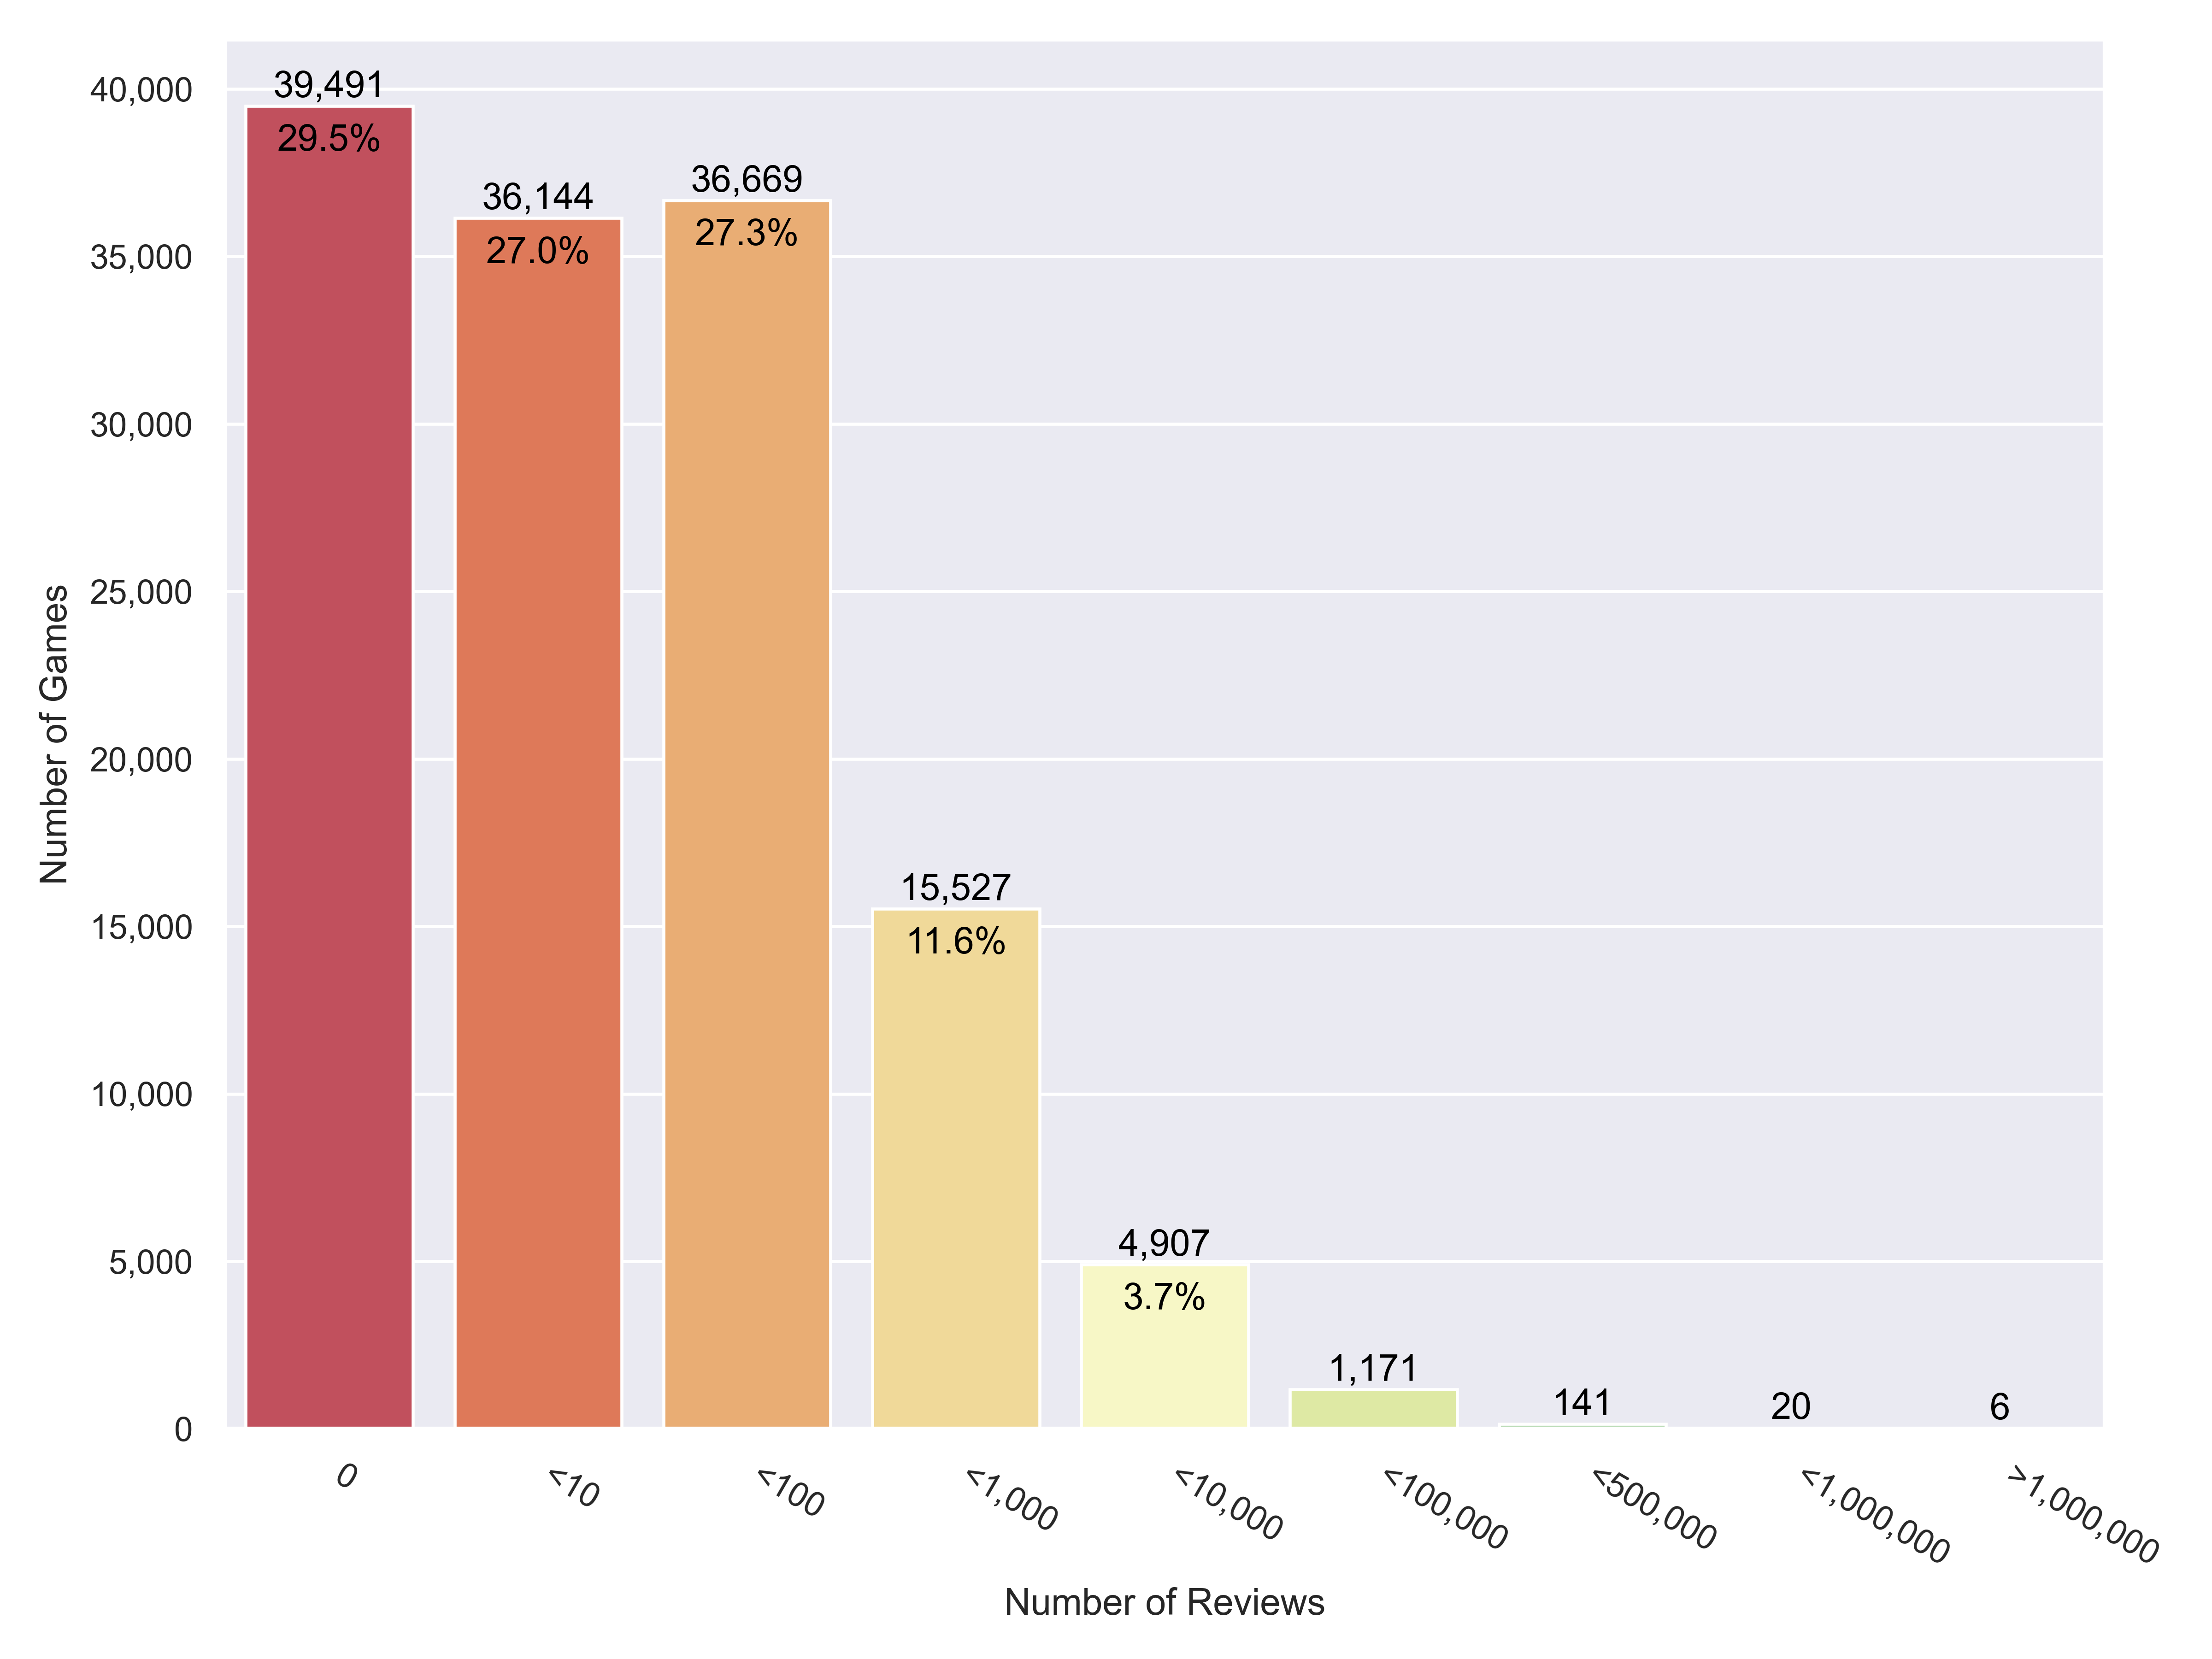
\includegraphics[width=\textwidth]{data/results/plots/review_plot}
    \caption{Distribution of Reviews Across Games}
    \label{fig:review_fig}
\end{figure}


\subsection{Reviews}\label{subsec:reviews}
Among all these games the numbers of reviews for each game are not evenly distributed, as was expected.
The biggest portion of games do not have reviews at all, while some games have more than one million reviews.
These reviews also vary strongly in their length but all withing the dimensions set by Steam which needs a review to
be between 5 and 8,000 characters.
The Steam API returns reviews as batches in a JSON format containing the reviews along with some anonymous meta data
about the author and the review.
For some basic metrics of the reviews see table~\ref{tab:review_metrics}.

\begin{table}[h]
    \centering
    \begin{tabular}{r|r|r}
    & Total & Only English\\\hline
        Reviews                 & 100,855,789 & 46,616,033\\
        Tokens                  & 15,023,225,453 & 10,643,950,482\\
        Mean Review Size        & 148.96 & 228.33\\
        Median Review Size      & 20 & 59
    \end{tabular}
    \caption{Review Metrics}
    \label{tab:review_metrics}
\end{table}


\subsection{Genres}\label{subsec:genres}
The term genre is used very loosely in this paper.
On Steam, users have the ability to give tags or key words to games or to upvote tags that are already given to that
game, incrementing the tags counter.
Through this mechanic, games have a list of user given tags along with the number of users that have given or upvoted
a tag.
If a game has more than 20 tags associated with it, only the 20 most common tags will be displayed on Steam.
While most tags correspond to traditional genre labels (e.g. adventure, strategy, RPG) some of them focus more on
features that could be present in any genre (e.g.\ early access, free to play, VR). There are also tags where it is
not entirely clear whether they correspond to a genre or not (e.g.\ indie, exploration, casual) because of the fluidity
of emerging new genres and subgenres.
To avoid biased selection this paper will call all user generated tags genres.
Further sampling and clustering of these tags into more traditional genres is always possible for future research at a
later date.
See table~\ref{tab:genre_metrics} for an overview of genres that are found within the 5 most common genres of all games
in the corpus.

\begin{figure}
    \centering
    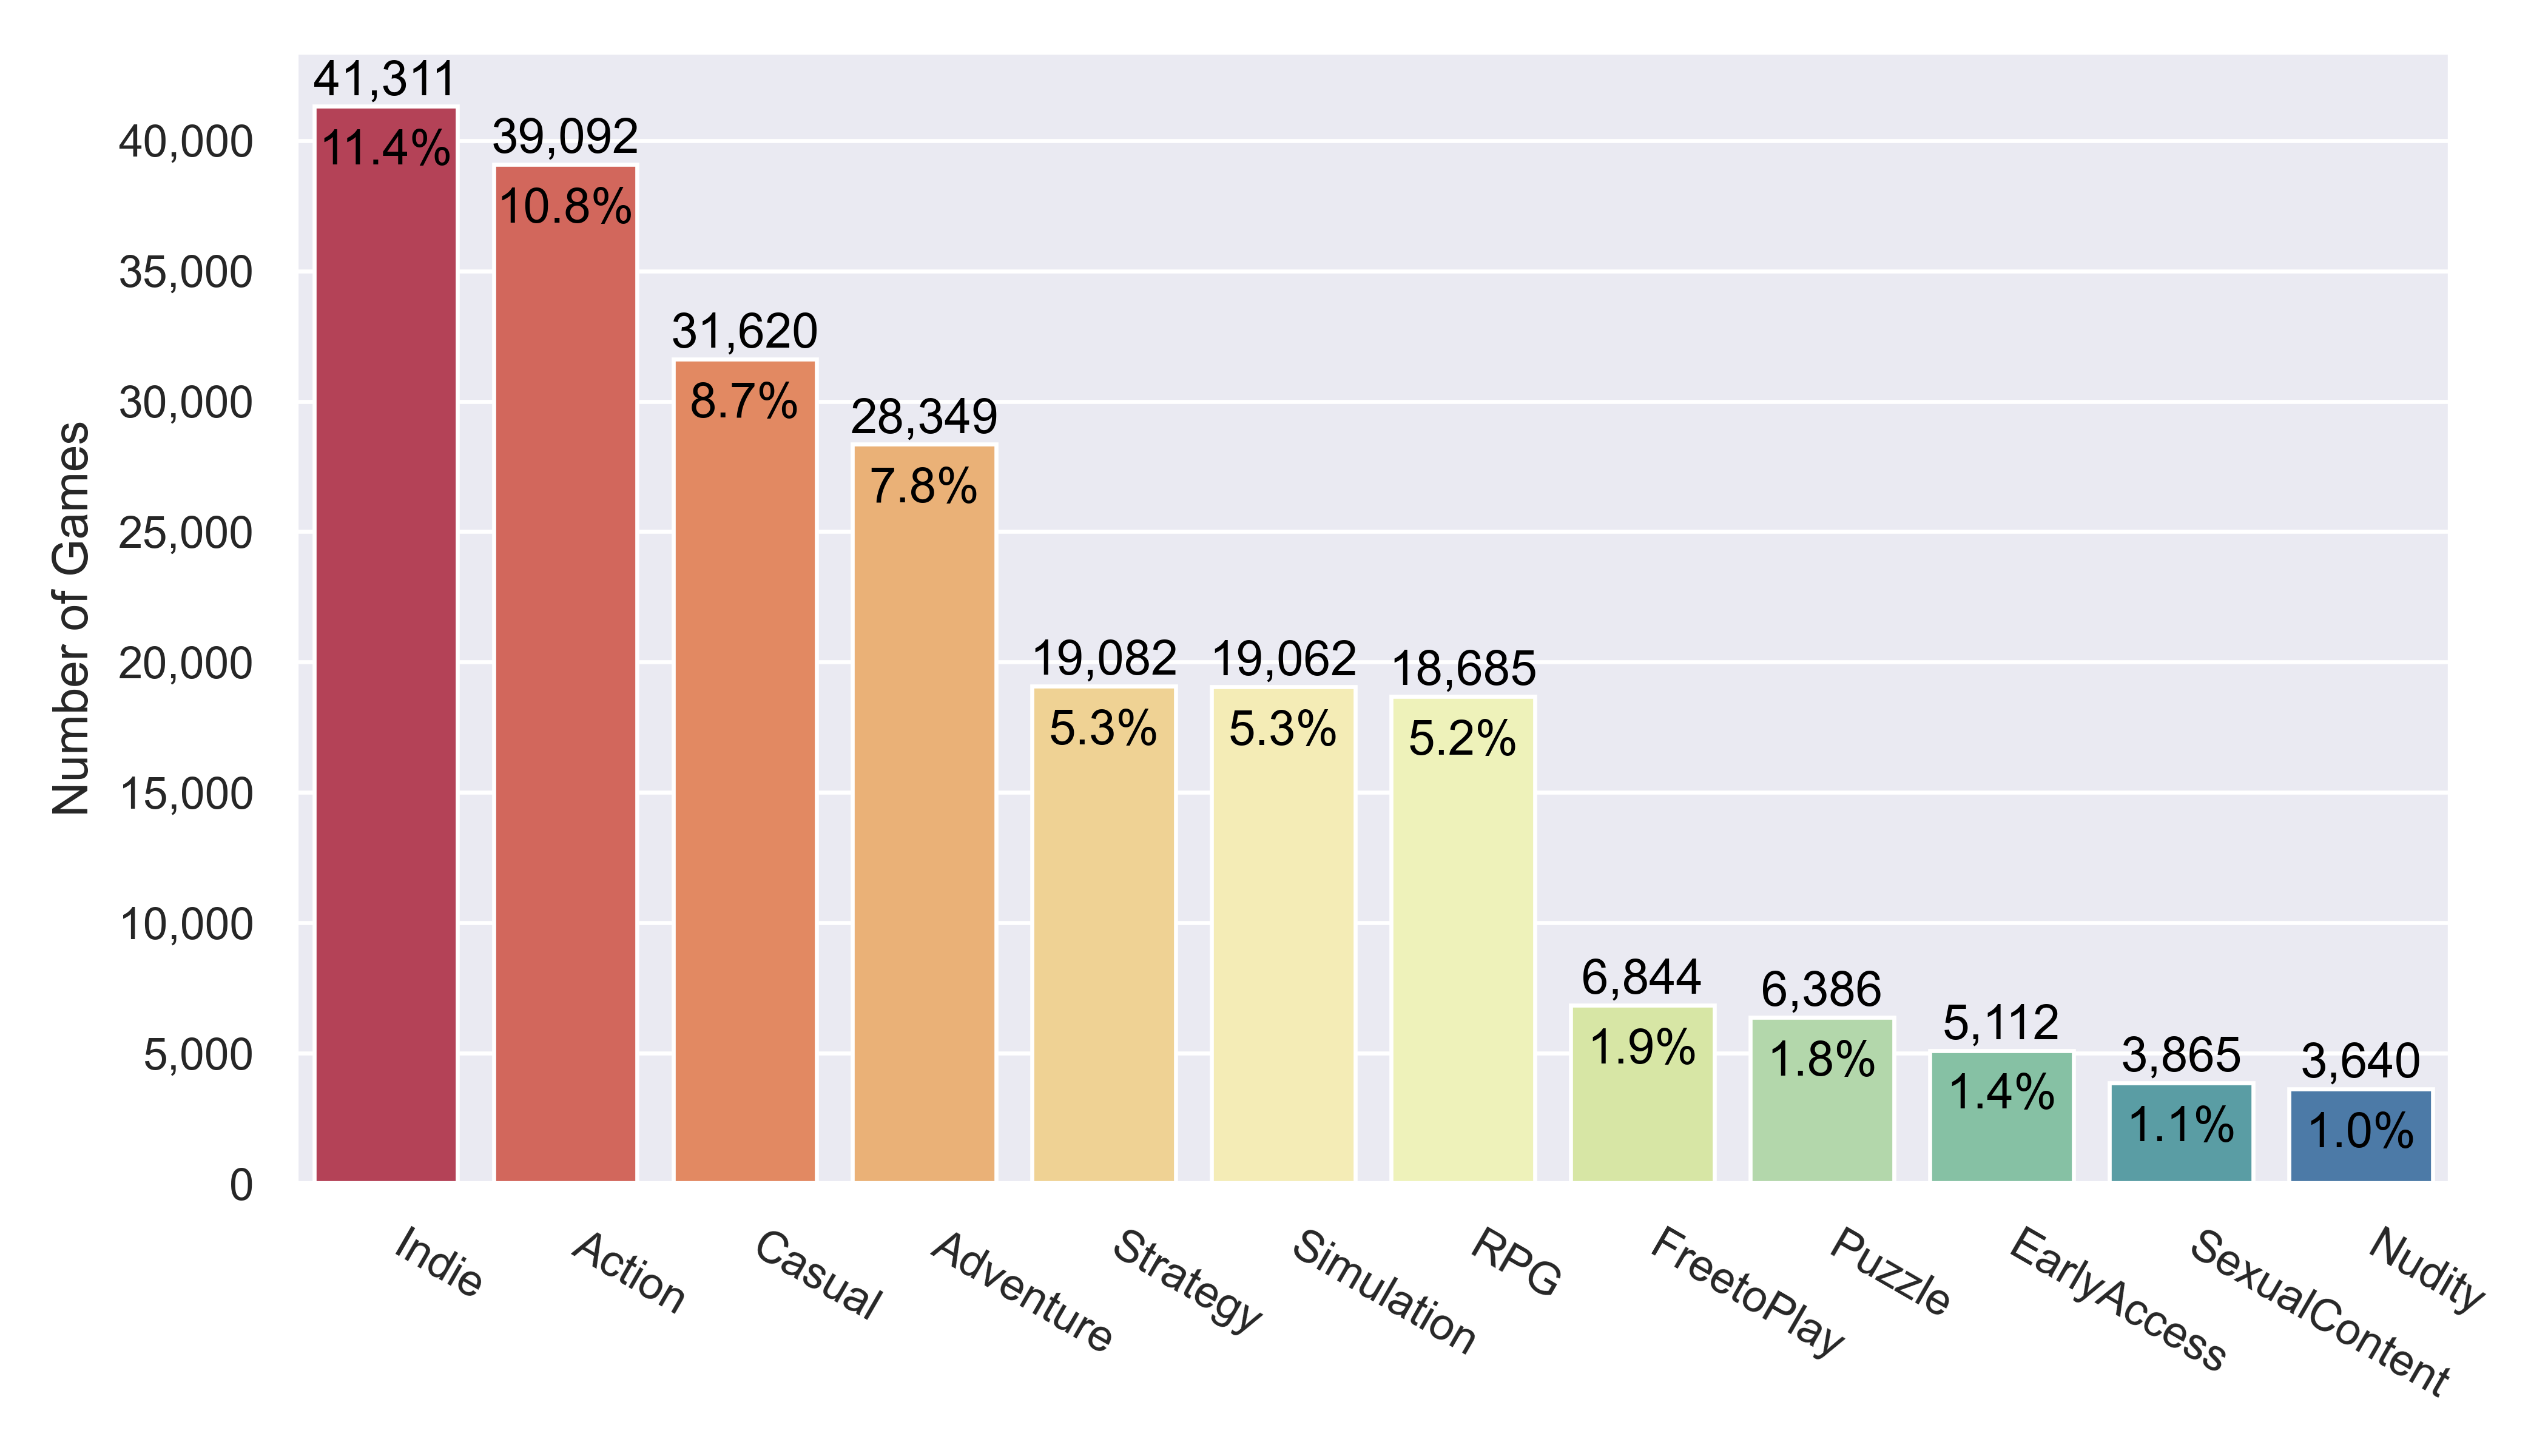
\includegraphics[width=\textwidth]{data/results/plots/tags_plot}
    \caption{Number of Games for the Ten Most Common Genres}
    \label{fig:tags_fig}
\end{figure}

\begin{table}[h]
    \centering
    \begin{tabular}{l|l}
    Genre Tag & Count\\\hline
        Indie & 41,311 \\
        Action & 39,092 \\
        Casual & 31,620 \\
        Adventure & 28,349 \\
        Strategy & 19,082 \\
        Simulation & 19,062 \\
        RPG & 18,685 \\
        FreetoPlay & 6,844 \\
        Puzzle & 6,386 \\
        EarlyAccess & 5,112 \\
        SexualContent & 3,865 \\
        Nudity & 3,640 \\
        Racing & 3,554 \\
        Sports & 3,481 \\
        Arcade & 2,800 \\
        VR & 2,771 \\
        Exploration & 2,767 \\
        Horror & 2,587 \\
        Design \& Illustration & 2,538 \\
        Platformer & 2,402
    \end{tabular}
    \caption{Distribution of the 20 Most Common Genres Across All Games}
    \label{tab:genre_metrics}
\end{table}



\section{Experimental design}\label{sec:experimental-design}
% how was the method overview specifically implemented (sampling algorithm, tf-idf using spacy medium model,
% implementation of smote and smote-enn, implementation of models, weights, ...)
% problems and challenges (no connection between people reviewing and people tagging besides assumed statistic
% connection)
% possible restrictions in interpreting the results (is it really the lexical features that the model learns? maybe
% check highest tf-idf values for each genre)
\subsection{Corpus generation}\label{subsec:corpus-generation}
The review data was gathered utilising Python scripts\footnote{See the repository linked on the front page for access
to all scripts and code used.} along with the Steam API. The genre data was not part of the Steam API and was therefore
crawled through a custom script accessing each games page on the Steam website and downloading its HTML content for
scraping in a later step.
Review and genre data has been combined by saving it in a custom database storing information like game id, review id,
review text and most common genre tags for every review for faster speeds when creating data samples.
These samples were created with multiple restrictions to attain as much balance as possible while using as much data as
possible.
Only games were included that had at least 10 reviews and each review was randomly chosen and had to be between 20 and
1000 token while collecting maximum of 1000 reviews per game.
Collected reviews where tokenised, cleaned from stop words and custom stop words, special characters and any other
noise like ASCII art, and then lemmatised.
Custom stop words were collected through comparison of most prominent token in earlier corpora using TF-IDF scores
among all genres present in the corpora.
The 50 most common tokens for all genres have been collected and counted.
Among these token, only those present in at least three genres have been removed.
Those consisted mostly of tokens belonging to review as a text genre like \textit{recommend}, \textit{feel} or
\textit{like} or of very generic adjectives like \textit{good}, \textit{bad} or \textit{fun}.
Tokens belonging to the broad field of video games like \textit{game} or \textit{play} were also added to the custom
stop words.
Content-specific words like \textit{level} or \textit{gameplay}, however, have not been removed.
For a full list of all custom stop words that were removed see appendix~\ref{sec:stops}.
TF-IDF vectors were created off the cleaned reviews and then corrected for imbalances using Synthetic Minority
Oversampling Technique (SMOTE), since although the same amount of review texts has been selected, the average text
length differed slightly in each genre label.
SMOTE was able to correct the imbalances by raising the minority classes to the same level as the majority classes by
introducing slight amounts of synthetic data.
The results were then passed on to training.

\subsection{Model training}\label{subsec:model-training}
The already prepared dataset was separated into TF-IDF vectors and genre labels, and a 80/20 split has been performed
for separating the training from the test set.
Multiple classifier models were trained, including Naive Bayes, Logistic Regression, Random Forest and Support Vector
Machine.
After training, relevant metrics like accuracy, recall, precision and F1 score were collected.




\section{Results and discussion}\label{sec:results-and-discussion}
% discuss results
% interprete ml metrics and how they relate to the research question
% interprete relation of metrics to linguistic features
% give some outline on future research
\begin{table}[h]
    \centering
    \begin{tabular}{r|r|r|r|r|r|r}
        & Average & Adventure & Strategy & Simulation & RPG & Puzzle \\\hline
        Recall      & 0.68 & 0.55 & 0.69 & 0.68 & 0.73 & 0.74\\
        Precision   & 0.68 & 0.6 & 0.71 & 0.66 & 0.65 & 0.75\\
        F1 Score    & 0.68 & 0.58 & 0.7 & 0.67 & 0.69 & 0.74\\
        Support     & 50000.0 & 10000.0 & 10000.0 & 10000.0 & 10000.0 & 10000.0
\end{tabular}
    \caption{Classifier Model Metrics for Naive Bayes}
    \label{tab:model_metrics}
\end{table}
\begin{table}[h]
    \centering
    \begin{tabular}{r|r|r|r|r|r|r}
        & Average & Adventure & Strategy & Simulation & RPG & Puzzle \\\hline
        Recall      & 0.68 & 0.57 & 0.71 & 0.68 & 0.7 & 0.76\\
        Precision   & 0.68 & 0.59 & 0.71 & 0.67 & 0.71 & 0.73\\
        F1 Score    & 0.68 & 0.58 & 0.71 & 0.68 & 0.7 & 0.74\\
        Support     & 50000.0 & 10000.0 & 10000.0 & 10000.0 & 10000.0 & 10000.0
\end{tabular}
    \caption{Classifier Model Metrics for Logistic Regression}
    \label{tab:model_metrics_logistic_regression}
\end{table}
\begin{table}[h]
    \centering
    \begin{tabular}{r|r|r|r|r|r|r}
        & Average & Adventure & Strategy & Simulation & RPG & Puzzle \\\hline
        Recall      & 0.68 & 0.54 & 0.71 & 0.68 & 0.71 & 0.76\\
        Precision   & 0.68 & 0.61 & 0.7 & 0.66 & 0.7 & 0.72\\
        F1 Score    & 0.68 & 0.58 & 0.7 & 0.67 & 0.7 & 0.74\\
        Support     & 50000.0 & 10000.0 & 10000.0 & 10000.0 & 10000.0 & 10000.0
\end{tabular}
    \caption{Classifier Model Metrics for Support Vector Machine}
    \label{tab:model_metrics}
\end{table}
\begin{table}[h]
    \centering
    \begin{tabular}{r|r|r|r|r|r|r}
        & Average & Adventure & Strategy & Simulation & RPG & Puzzle \\\hline
        Recall      & 0.62 & 0.51 & 0.61 & 0.63 & 0.64 & 0.7\\
        Precision   & 0.62 & 0.49 & 0.66 & 0.6 & 0.65 & 0.7\\
        F1 Score    & 0.62 & 0.5 & 0.64 & 0.61 & 0.64 & 0.7\\
        Support     & 50000.0 & 10000.0 & 10000.0 & 10000.0 & 10000.0 & 10000.0
\end{tabular}
    \caption{Classifier Model Metrics for Random Forest}
    \label{tab:model_metrics}
\end{table}
\begin{table}[h]
    \centering
    \begin{tabular}{r|r|r|r|r|r}
         & Naive Bayes & Logistic Regression & Random Forest & SVM & Aggregated \\\hline
        Accuracy    & 0.68 & 0.68 & 0.62 & 0.68 & 0.67\\
        Recall      & 0.68 & 0.68 & 0.62 & 0.68 & 0.67\\
        Precision   & 0.68 & 0.68 & 0.62 & 0.68 & 0.67\\
        F1 Score    & 50000.0 & 50000.0 & 50000.0 & 50000.0 & 50000.0
\end{tabular}
    \caption{Aggregated Classifier Model Metrics}
    \label{tab:model_metrics}
\end{table}
\begin{table}[h]
    \centering
    \begin{tabular}{r|r|r|r|r|r}
        Adventure & Strategy & Simulation & RPG & Puzzle \\
        \hline
        story,  0.25  & units,  0.15  & route,  0.15  & story,  0.2  & levels,  0.22  \\
        short,  0.13  & strategy,  0.14  & vr,  0.15  & combat,  0.16  & level,  0.17  \\
        music,  0.11  & tower,  0.12  & work,  0.12  & characters,  0.13  & story,  0.16  \\
        gameplay,  0.11  & ai,  0.11  & better,  0.11  & character,  0.12  & music,  0.14  \\
        characters,  0.11  & gameplay,  0.11  & buy,  0.11  & hours,  0.11  & simple,  0.12  \\
        graphics,  0.1  & cards,  0.1  & real,  0.1  & gameplay,  0.11  & easy,  0.12  \\
        level,  0.1  & campaign,  0.1  & things,  0.09  & system,  0.1  & gameplay,  0.11  \\
        experience,  0.1  & defense,  0.1  & money,  0.09  & better,  0.1  & short,  0.11  \\
        art,  0.1  & turn,  0.1  & price,  0.09  & far,  0.09  & hours,  0.1  \\
        point,  0.09  & hours,  0.1  & experience,  0.09  & world,  0.09  & hard,  0.09  \\
        interesting, 0.09 & card, 0.1 & free, 0.08 & buy, 0.09 & art, 0.09 \\
        controls, 0.09 & better, 0.09 & graphics, 0.08 & interesting, 0.09 & achievements, 0.09 \\
        price, 0.09 & buy, 0.09 & train, 0.08 & content, 0.08 & price, 0.09 \\
        better, 0.08 & player, 0.09 & add, 0.08 & enemies, 0.08 & mechanics, 0.09 \\
        character, 0.08 & war, 0.08 & sim, 0.08 & things, 0.08 & challenging, 0.09 \\
        $\vdots$ & $\vdots$ & $\vdots$ & $\vdots$ & $\vdots$ & $\vdots$
    \end{tabular}
    \caption{Tokens with TF-IDF Scores by Genre}
    \label{tab:tfidf_by_genre}
\end{table}
\begin{table}[h]
    \centering
    \begin{tabular}{l|c|c|c|c|c}
        Token & Adventure & Strategy & Simulation & RPG & Puzzle \\
        \hline
        story & 0.25 & - & 0.06 & 0.2 & 0.16 \\
        gameplay & 0.11 & 0.11 & 0.06 & 0.11 & 0.11 \\
        hours & 0.08 & 0.1 & 0.07 & 0.11 & 0.1 \\
        better & 0.08 & 0.09 & 0.11 & 0.1 & 0.07 \\
        level & 0.1 & 0.08 & - & 0.08 & 0.17 \\
        buy & 0.07 & 0.09 & 0.11 & 0.09 & 0.06 \\
        graphics & 0.1 & 0.08 & 0.08 & 0.07 & 0.08 \\
        price & 0.09 & 0.07 & 0.09 & 0.07 & 0.09 \\
        work & 0.07 & 0.08 & 0.12 & 0.07 & 0.06 \\
        things & 0.08 & 0.07 & 0.09 & 0.08 & 0.07
    \end{tabular}
    \caption{10 Most Prominent Tokens with TF-IDF Scores across Genres}
    \label{tab:prominent_tokens}
\end{table}

\begin{figure}
    \centering
    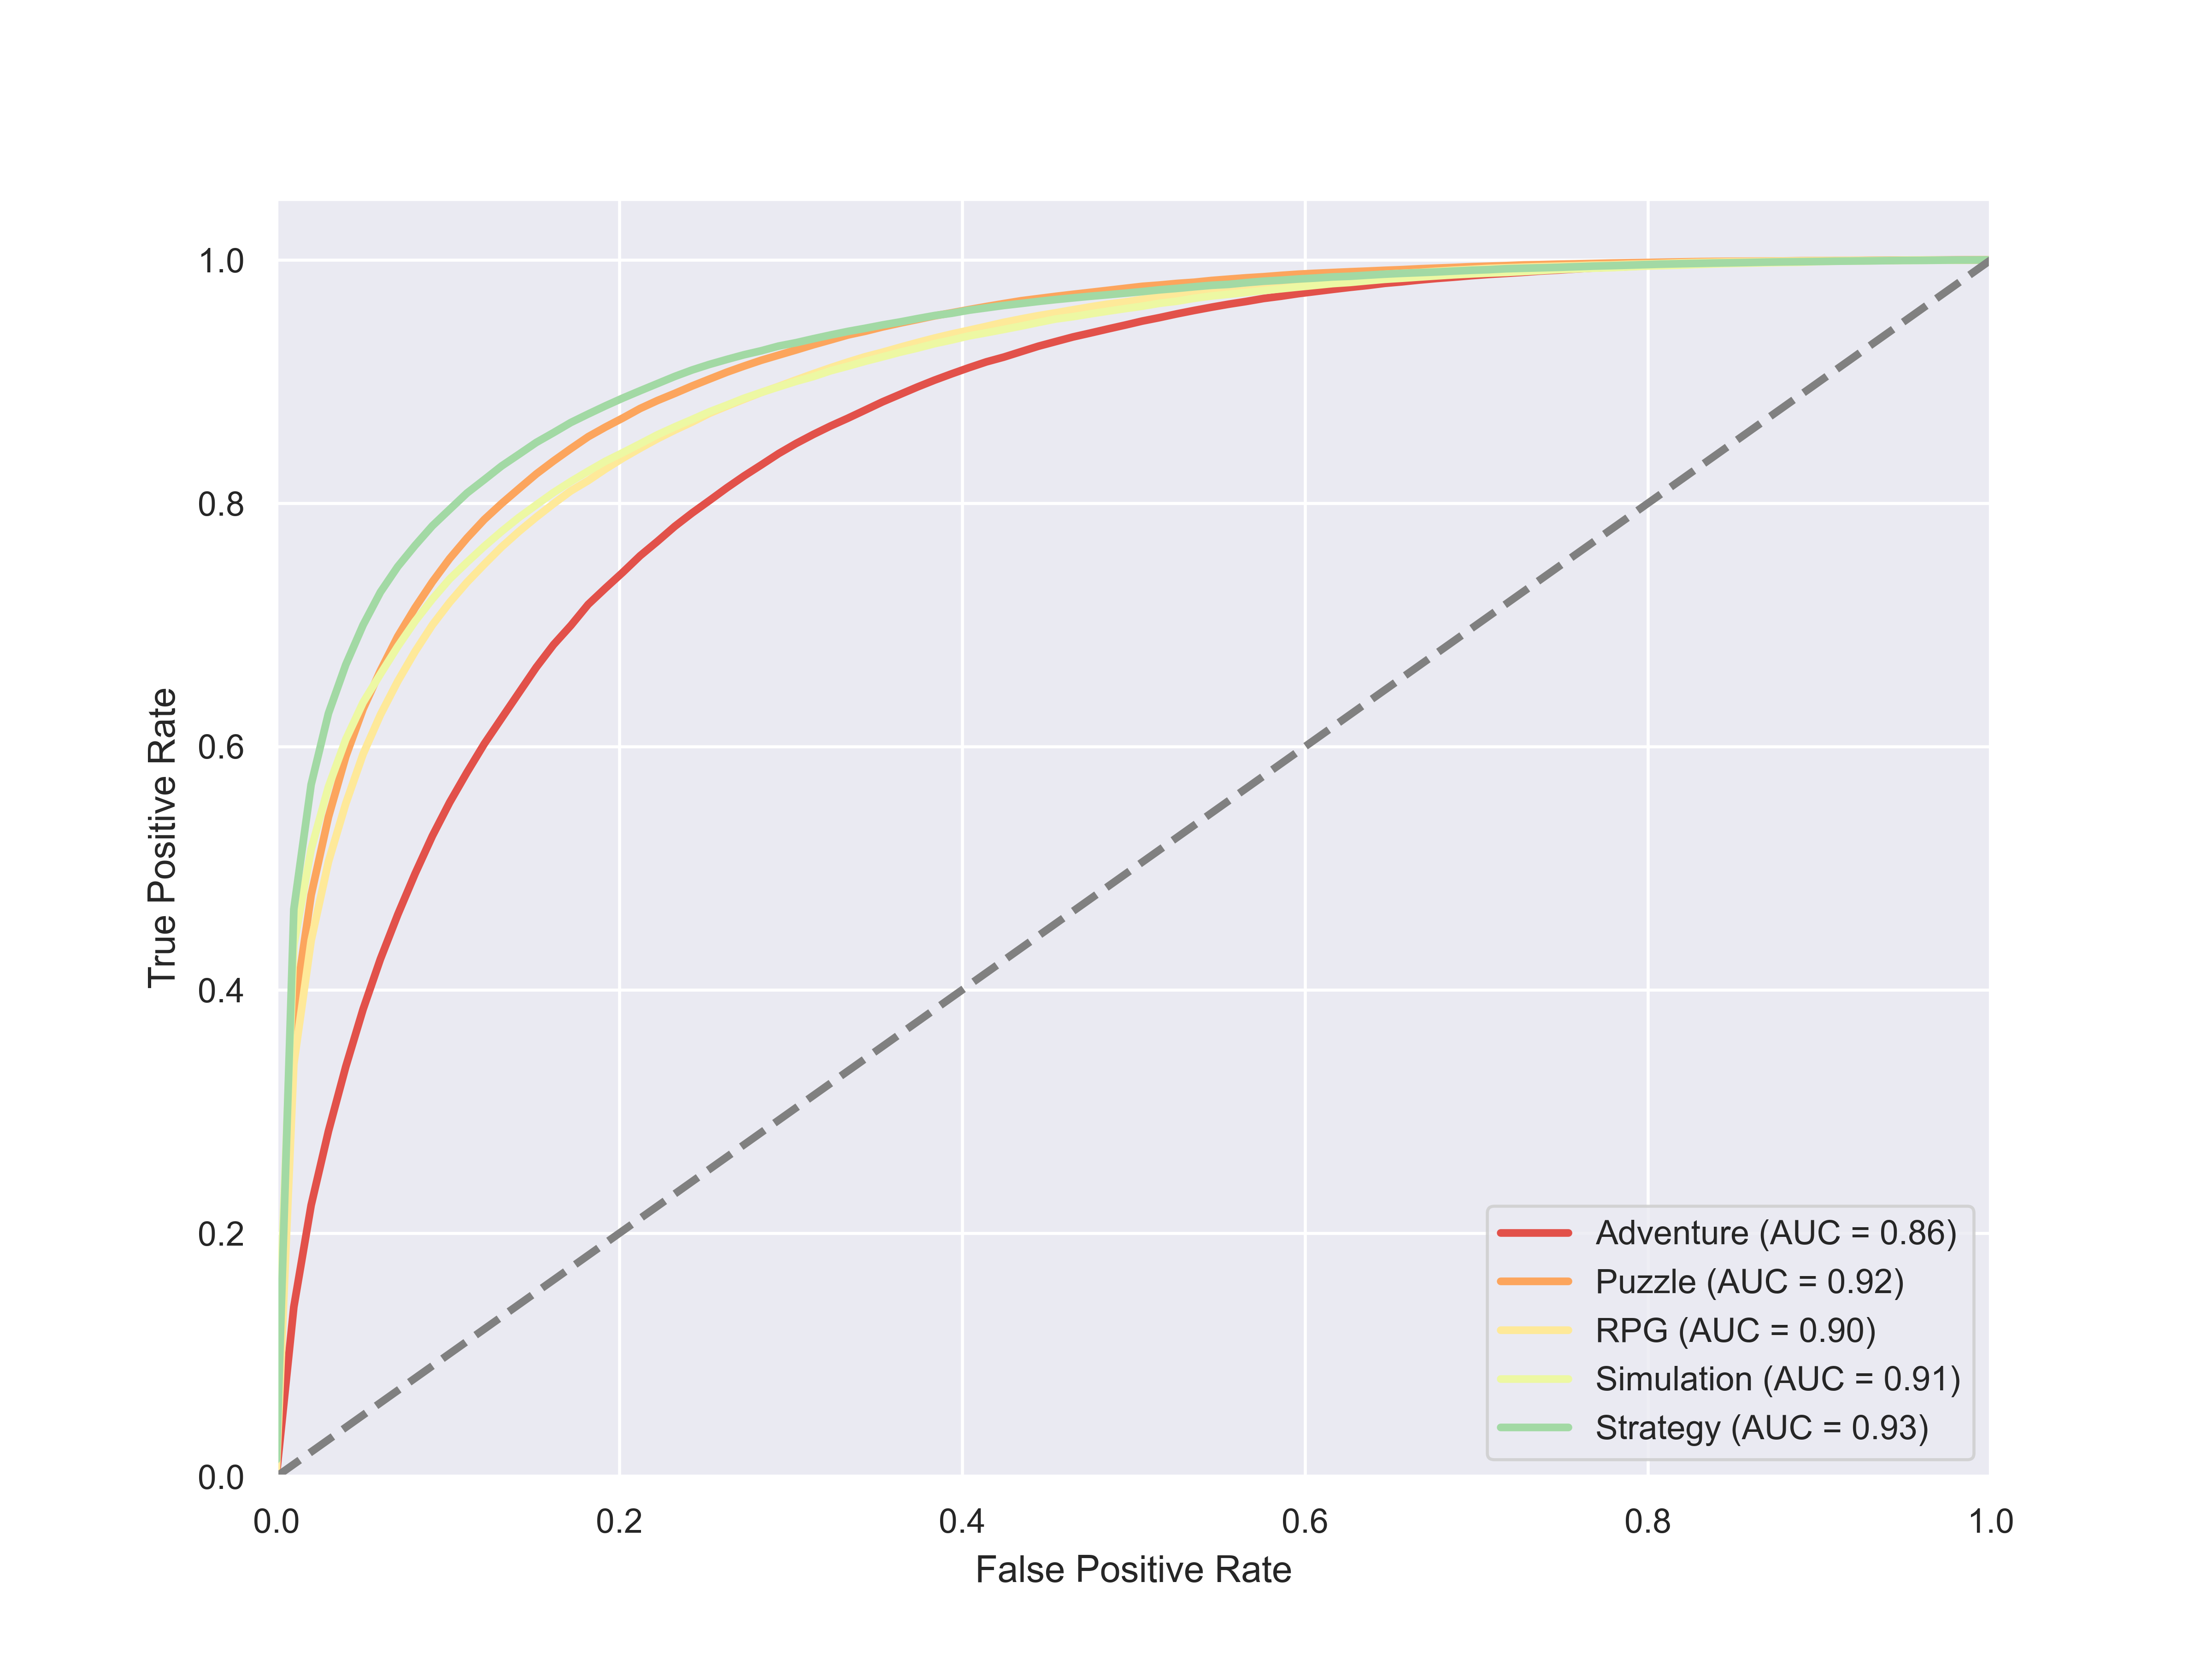
\includegraphics[width=\textwidth]{data/results/plots/naive_bayes_roc}
    \caption{ROC Curve OvR for Naive Bayes}
    \label{fig:nb_roc_fig}
\end{figure}


\begin{figure}
    \centering
    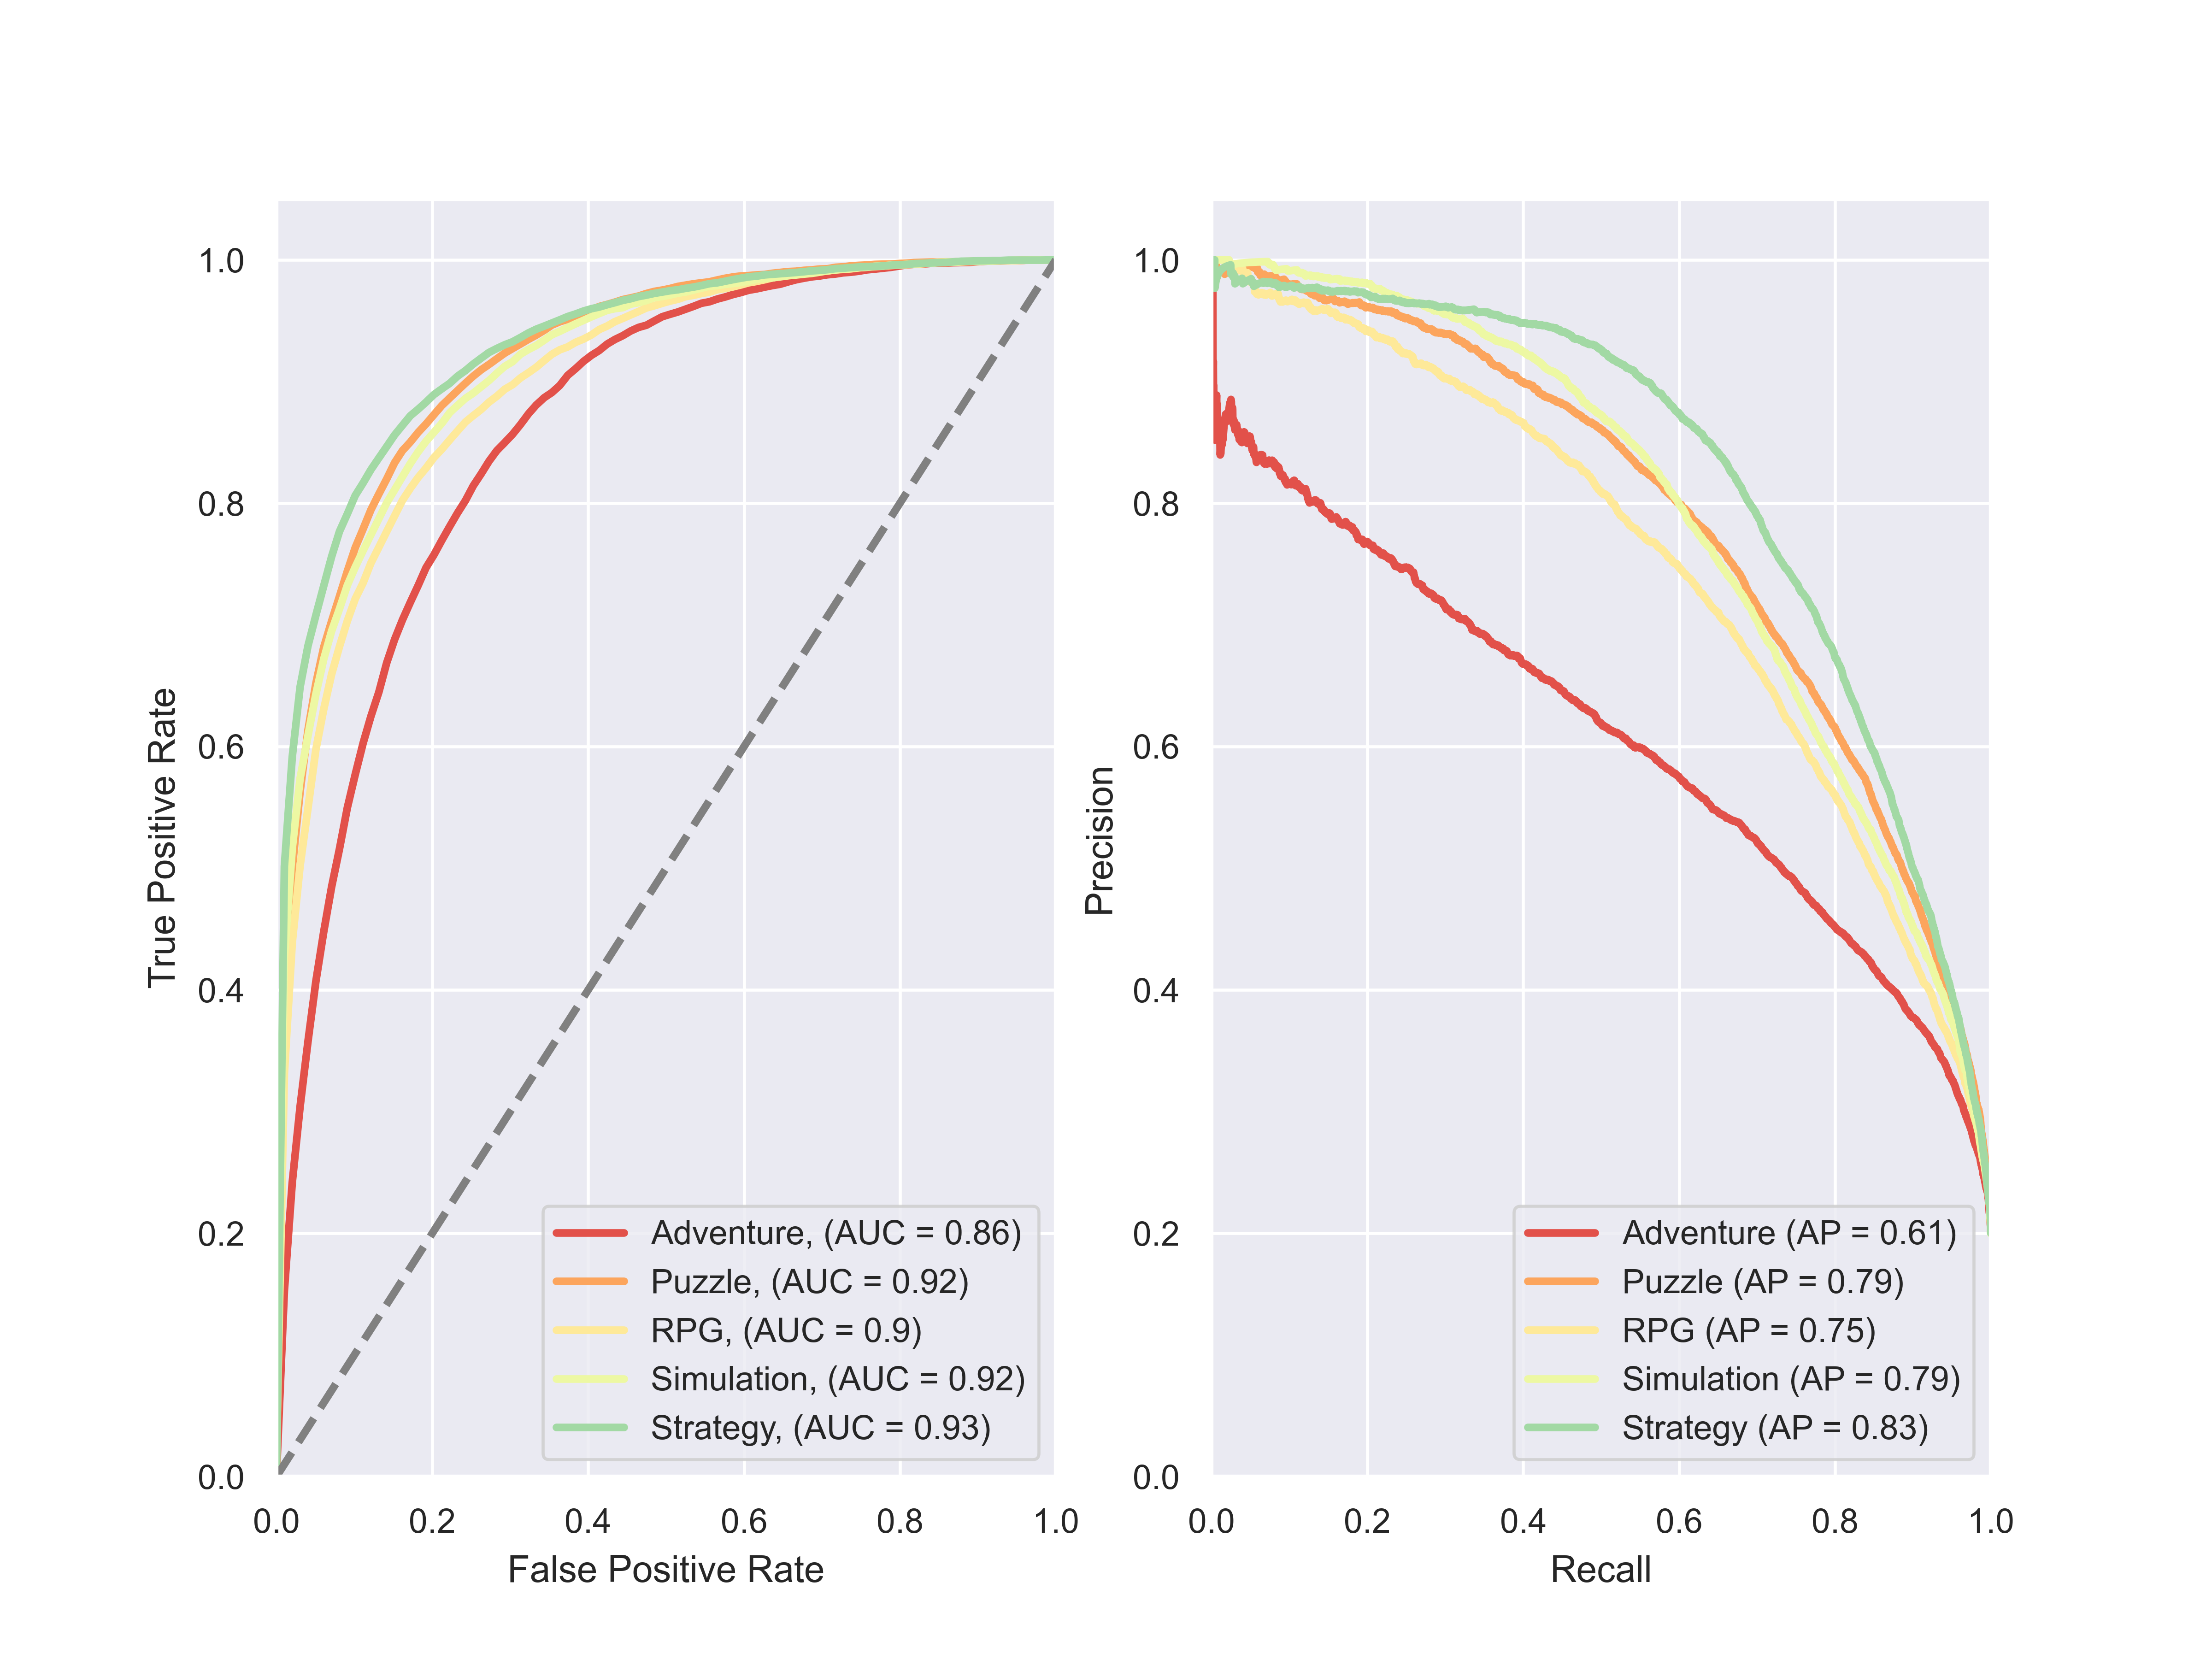
\includegraphics[width=\textwidth]{data/results/plots/logistic_regression_roc}
    \caption{ROC Curve OvR for Logistic Regression}
    \label{fig:lr_roc_fig}
\end{figure}


\begin{figure}
    \centering
    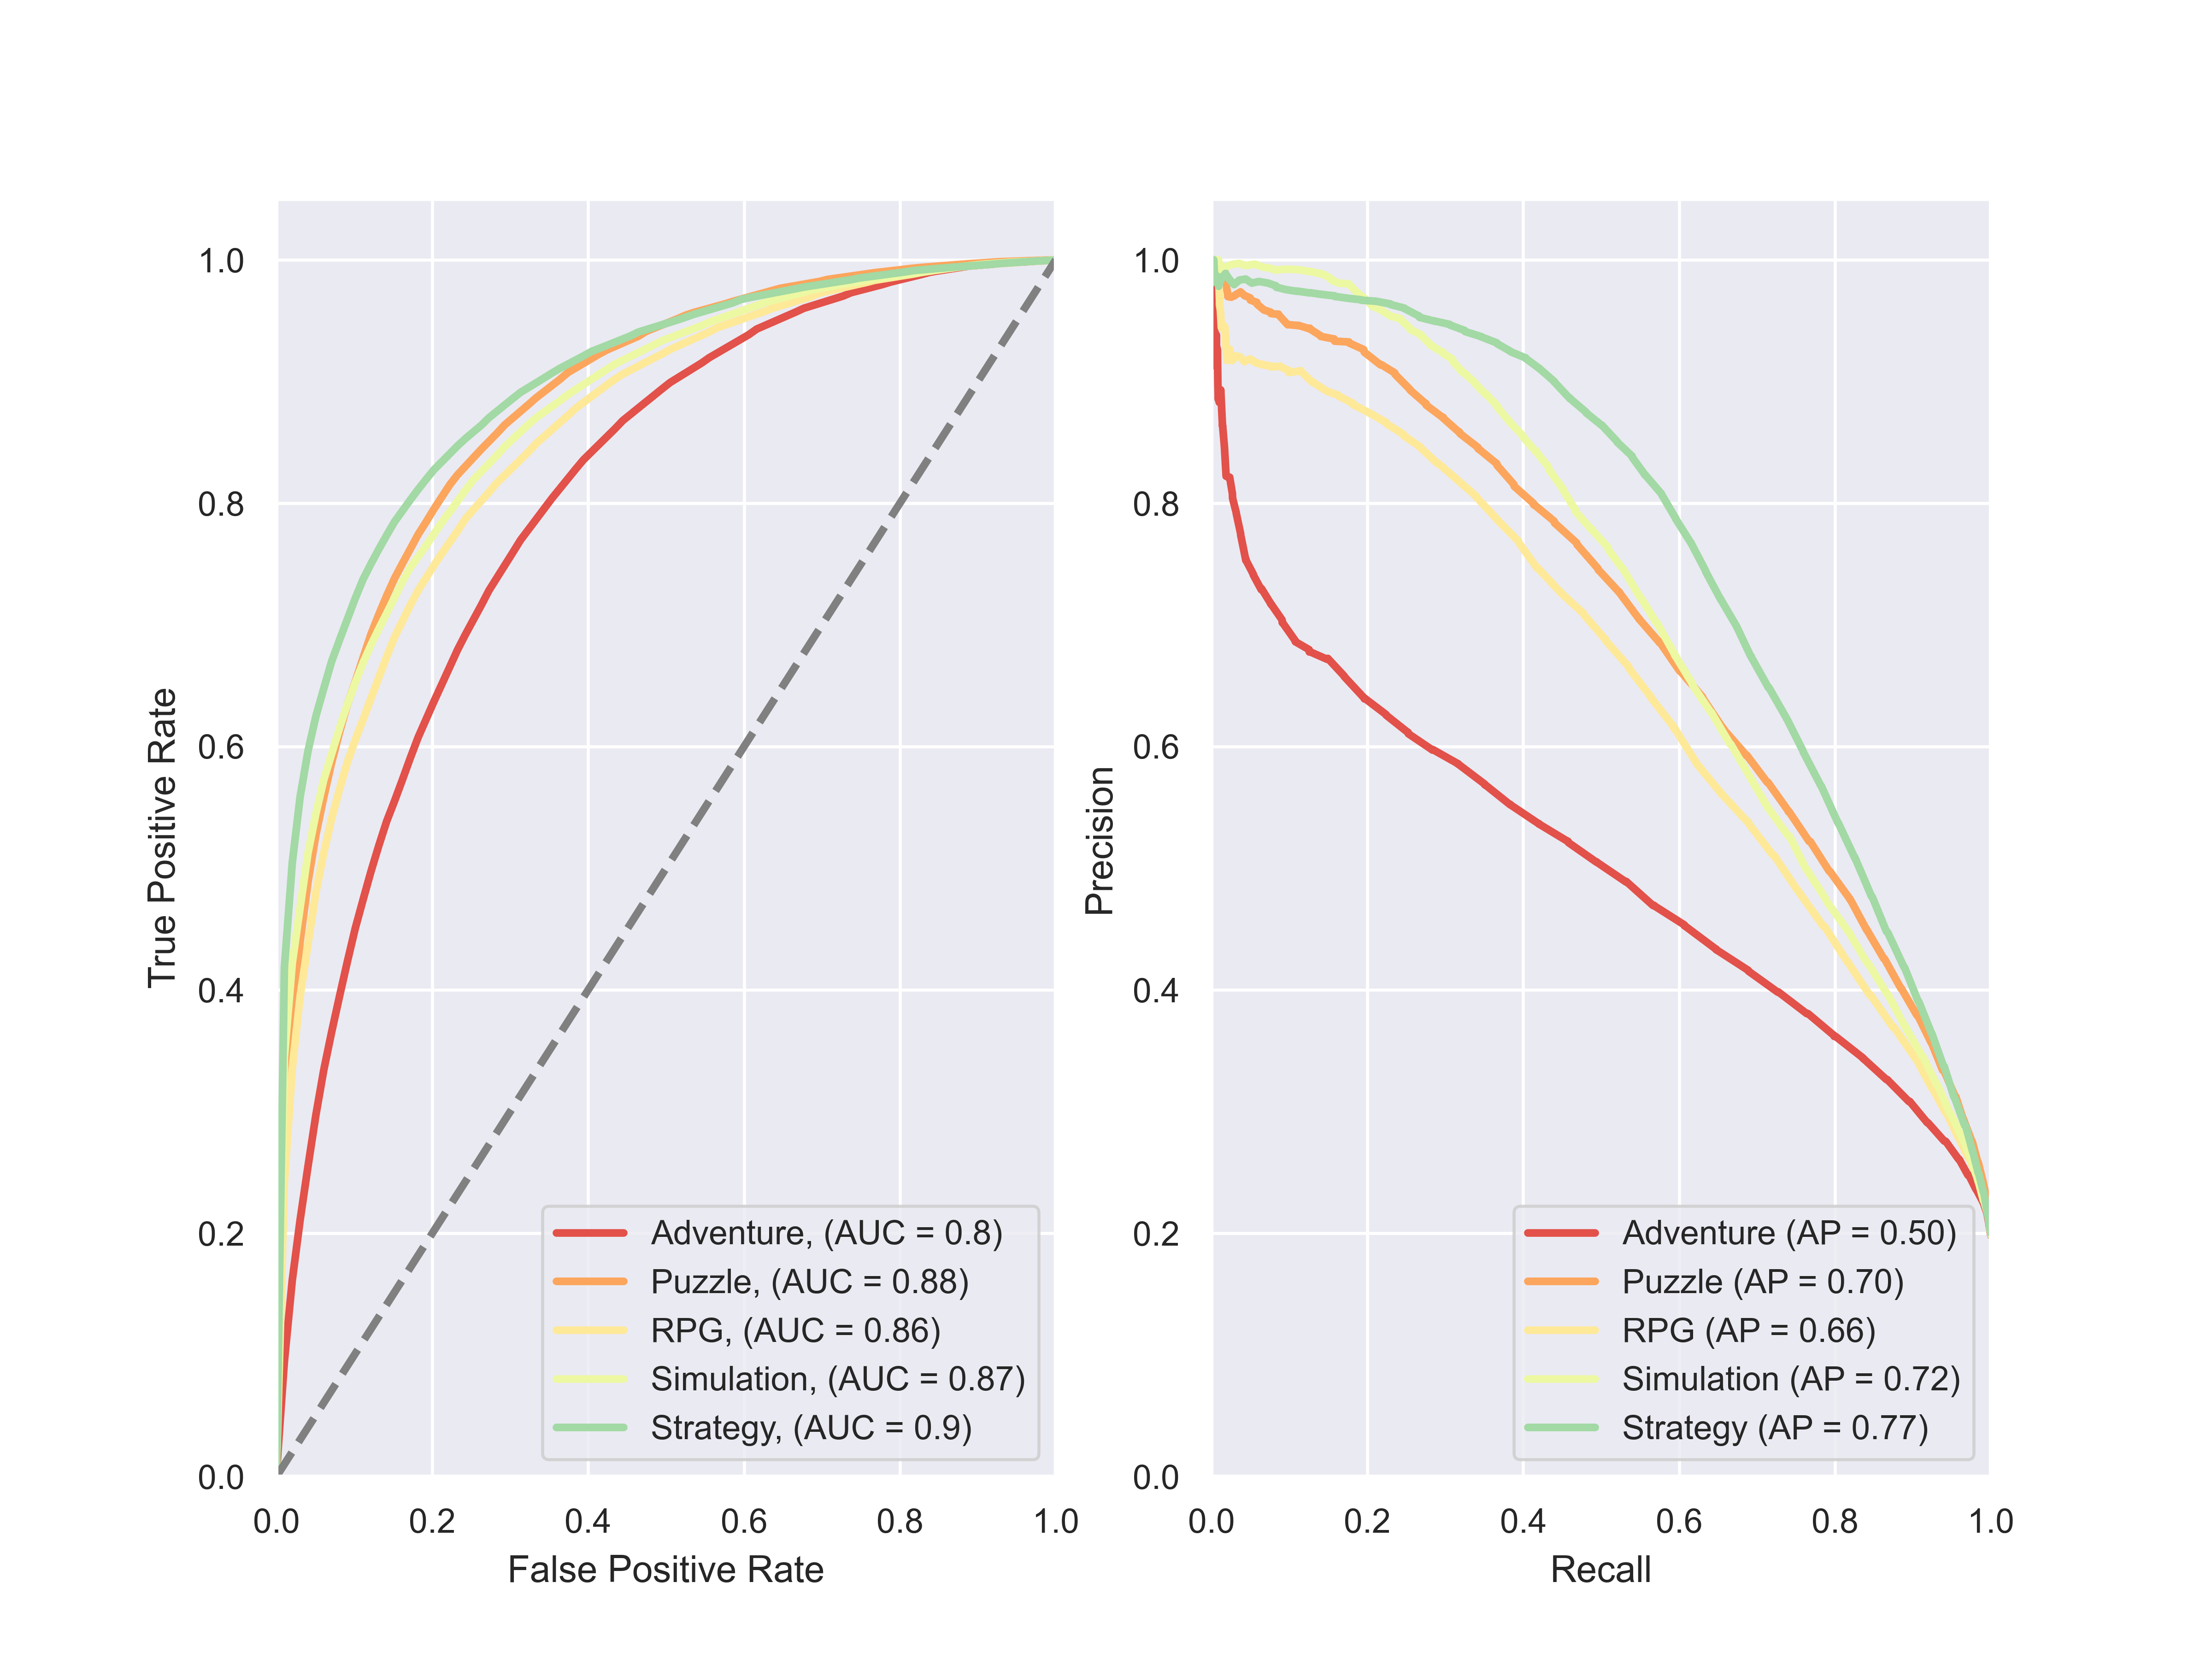
\includegraphics[width=\textwidth]{data/results/plots/random_forest_roc}
    \caption{ROC Curve OvR for Random Forest}
    \label{fig:rf_roc_fig}
\end{figure}



\section{Conclusion}\label{sec:conclusion}
% sum stuff up


\clearpage

\nocite{*}
\printbibliography

\clearpage

\begin{appendices}
\section{Custom stop words}\label{sec:stops}
Custom stop words that were removed from the corpora before model training:
\begin{itquote}
    game, like, good, games, time, play, fun, way, great, little, bit, lot, pretty, feel, think, recommend, playing,
    things, want, different, played, worth, got, love, better, new, need, find, bad, nice, steam, know, dlc, use, hours,
    people, nt\footnote{This is probably an artifact created by stemming the falsely written \textit{dont} (without
    apostrophe).}, adventure, strategy, simulation, rpg, puzzle
\end{itquote}
\end{appendices}



\end{document}    